\section{Results}

\subsection{ Multiplying two matrices with different sizes}
This section discusses the time taken both for parallelized and single thread  multiplying two matrices of the same size.
The test repeated the multiplication with the size of the matrix increasing each time.
The results of the multiplication are shown in figure \ref{fig:Single_thread_vs_Parallel_processing_time}.

\begin{figure}[H]
    \centering
    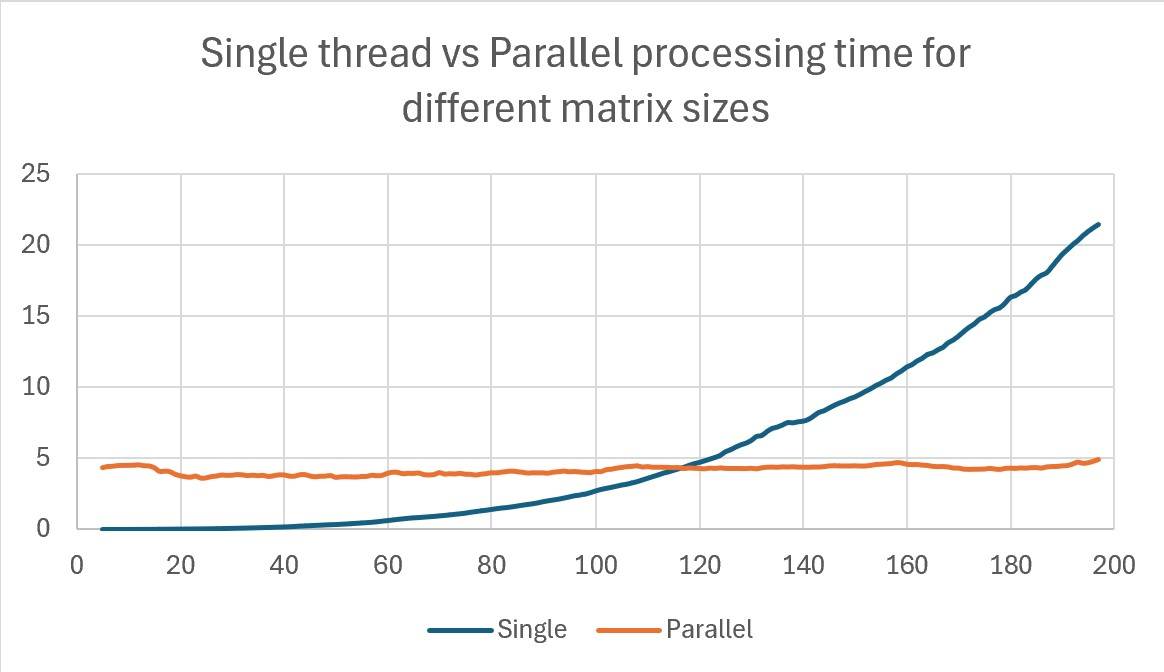
\includegraphics[width=1\columnwidth]{Figures/Single_thread_vs_Parallel_processing_time_for_different_matrix_sizes}
    \caption{Graph of single thread vs Parallel processing time for different matrix sizes}
    \label{fig:Single_thread_vs_Parallel_processing_time}
\end{figure}

The results show that the time taken for single-thread matrix multiplication is initially faster than parallelized multiplication up to size of the matrix around 117.
After size 117, parallelized multiplication becomes faster. This is indicated on the graph by time taken for the single thread processing increases with a larger exponential scale.
These results occur because the time due to overhead of setting up parallel processing is 4 ms which is larger than the time taken when running the program with small sized matrices on a single thread.
However, as the matrix size increases, the time taken for single-thread multiplication increases at a faster exponentially rate, resulting in longer processing time.

% should include a speed up graph here

\subsection{ Multiplying different number of matrices with same sizes}
This section discusses the time taken for parallelized verses single thread multiplying different numbers of matrices of the same size.

\begin{figure}[H]
    \centering
    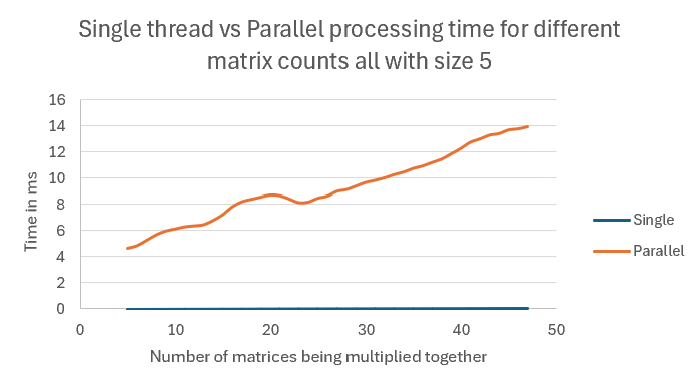
\includegraphics[width=1\columnwidth]{Figures/different_matrix_counts_size 5.png}
    \caption{Single thread vs Parallel processing time for different matrix counts all with size 10}
    \label{fig:different_matrix_counts_size 5}
\end{figure}

\begin{figure}[H]
    \centering
    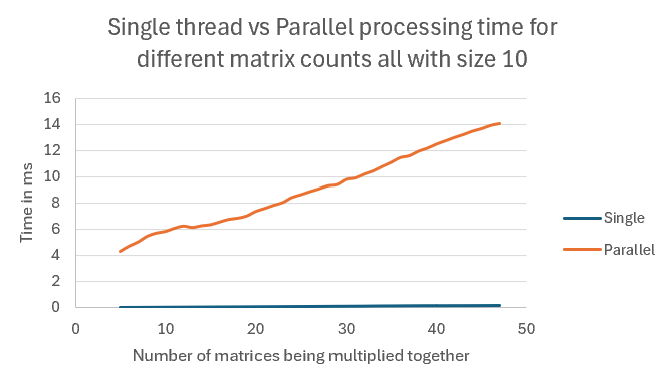
\includegraphics[width=1\columnwidth]{Figures/different_matrix_counts_size 10.png}
    \caption{Single thread vs Parallel processing time for different matrix counts all with size 10}
    \label{fig:different_matrix_counts_size 10}
\end{figure}

\begin{figure}[H]
    \centering
    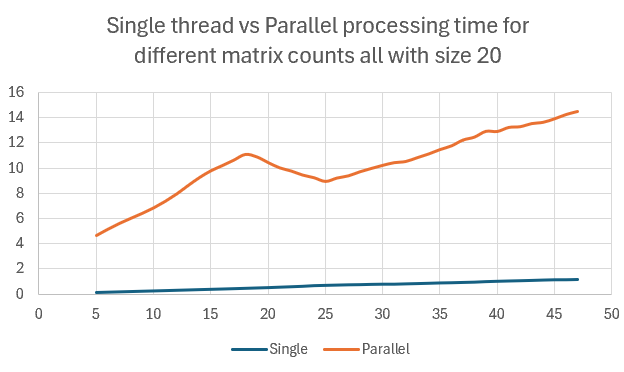
\includegraphics[width=1\columnwidth]{Figures/different_matrix_counts_size 20}
    \caption{Single thread vs Parallel processing time for different matrix counts all with size 20}
    \label{fig:different_matrix_counts_size 20}
\end{figure}

\begin{figure}[H]
    \centering
    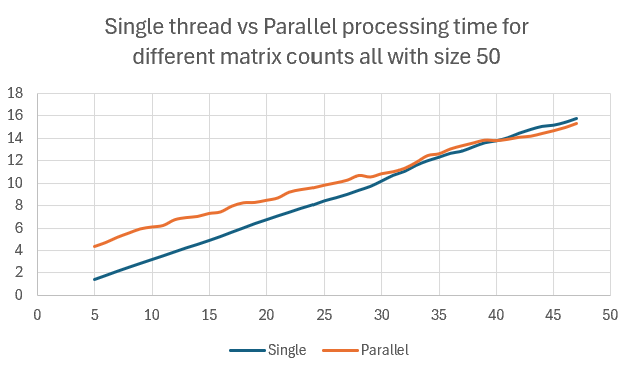
\includegraphics[width=1\columnwidth]{Figures/different_matrix_counts_size 50}
    \caption{Single thread vs Parallel processing time for different matrix counts all with size 50}
    \label{fig:different_matrix_counts_size 50}
\end{figure}

\begin{figure}[H]
    \centering
    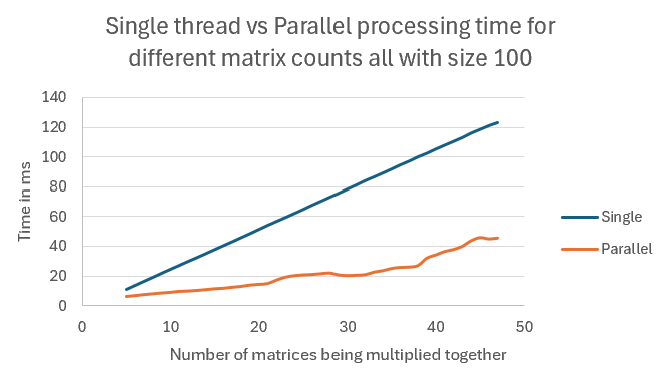
\includegraphics[width=1\columnwidth]{Figures/different_matrix_counts_size 100}
    \caption{Single thread vs Parallel processing time for different matrix counts all with size 100}
    \label{fig:different_matrix_counts_size 100}
\end{figure}

Looking at the results in figures: \ref{fig:different_matrix_counts_size 5}, \ref{fig:different_matrix_counts_size 10}, \ref{fig:different_matrix_counts_size 20}, \ref{fig:different_matrix_counts_size 50} and \ref{fig:different_matrix_counts_size 100},
It can be seen that there are two different types of over heads the openCl setup overheads and the overheads for starting the kernel.
The openCl setup overheads are the same for all the different matrix counts, this is because the openCl setup is done once and the same for all the different matrix counts.
This is indicated in our graph because the time taken at matrix count of 5 remain around 5ms independent of matrix size.

The overhead of starting the kernel to run seem to result in a linear increase in time  as the matrix count increases.
This occurs because each time the a new test is run a the buffer need to be re initialized and the kernel need to be started.
This can be seen in the graph because both the parallelized and single thread  result in linear increase in time as the matrix count increases.
however percentage of time spent parallelizing decreases as the matrix count increases.
This is indicated in the in figure \ref{fig:different_matrix_counts_size 50} where the linear graf of the time take vs matrix cont for parallelized multiplication
and single thread multiplication intersect. in other words there is an increase in efficiency of parallelized multiplication as the matrix count increases.

Looking at all the graph it can be seen that as the matrix size increases the speed up for parallelized multiplication vs the single thread multiplication improves.
In other words at smaller matrix sizes the time taken for parallelized multiplication is longer than the time taken for single thread multiplication
and at larger matrix sizes the time taken for parallelized multiplication is shorter than the time taken for single thread multiplication.




